\documentclass[usenames,dvipsnames]{beamer}
\usetheme[sectionpage=none]{metropolis}
\usepackage[T1]{fontenc}
\usepackage{amsmath, amssymb, amssymb, bbm}
\usepackage{mathtools}
\usepackage{hyperref}
\usepackage{marvosym}
\usepackage{alltt}
\usepackage{xcolor}
\usepackage{lmodern}
\usepackage{graphicx}
\usepackage{tikz}
\usepackage{verbatim}
\usetikzlibrary{arrows}

\newcommand{\R}{\mathbb{R}}
\newcommand{\N}{\mathbb{N}}
\newcommand{\Z}{\mathbb{Z}}
\newtheorem{prop}{Proposition}

\title{Submodular function minimisation}
\date[]{\today}
\author[S. Schenker]{Sebastian Schenker}

\begin{document}
\maketitle

\begin{frame}
  \tableofcontents
\end{frame}

\section{Motivation}
\begin{frame}{Steiner tree problem}
  \begin{center}
    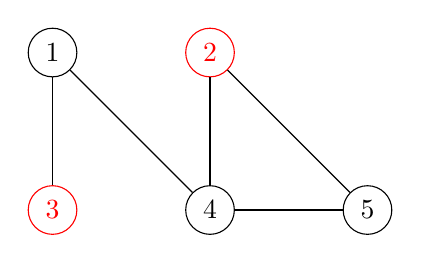
\begin{tikzpicture}[node distance = 2cm]
    \node[draw,circle](1) {$1$};
    \node[draw,circle, red](2) [right of=1] {$2$};
    \node[draw,circle, red](3) [below of=1] {$3$};
    \node[draw,circle](4) [right of=3] {$4$};
    \node[draw,circle](5) [right of=4] {$5$};
    \draw (1) -- (3);% node[midway,left] %{$e_{13}$};
    \draw (1) -- (4);% node[midway,above] {$e_{14}$};
    \draw[] (2) -- (4);% node[midway,right] {$e_{24}$};
    \draw[] (2) -- (5);% node[midway,below] {$e_{25}$};
    \draw[] (4) -- (5);% node[midway,below] {$e_{45}$};
    \end{tikzpicture}
    \end{center}
  \begin{itemize}
  \item given graph $G = (V,E)$, set of \textcolor{red}{terminals} $T \subseteq V$
  \item a Steiner tree is a tree spanning $T$
  \end{itemize}
\end{frame}

\begin{frame}{Steiner tree polytope}
  \begin{itemize}
  \item $x_e \in \{0,1\}$ for $e \in E$ with $x_e = 1$ iff  $e$ is used in Steiner tree
  \item let $N = V \setminus T$ be the set of non-terminals
  \item $y_i \in \{0,1\}$ for $i \in N$ iff vertex $i$ is spanned by the Steiner tree
  \item Steiner tree polytope (relaxation) $P \subset \R^{|E| + |N|}$:
  \end{itemize}
  \begin{align}
    \sum\limits_{e \in E} x_e &= \sum\limits_{i \in N} y_i + |T| - 1\\
    \sum\limits_{e \in E(S)} x_e &\leq \sum\limits_{i \in N \cap S} y_i + |T \cap S| -1 &&\forall S \subseteq V,~S \cap T \neq \emptyset\\
    \sum\limits_{e \in E(S)} x_e &\leq \sum\limits_{i \in S \setminus \{k\}} y_i &&\forall S \subseteq N,~k \in S\\
    x_e &\geq 0 &&\forall e \in E\\
    y_i & \leq 1 &&\forall i \in N
  \end{align}
\end{frame}

\section{Preliminaries}
%% \begin{frame}{Set functions}
%%   \begin{itemize}
%%   \item let $f : 2^U \rightarrow \R$ be a set function
%%   \end{itemize}
%%   \begin{definition}
%%     A set function $f : 2^U \rightarrow \R$ is non-decreasing
%%     if \[f(S) \leq f(T)\] for $S \subseteq T \subseteq U$.
%%   \end{definition}
%% \end{frame}

%% \begin{frame}{Set function minimisation problem}
%%   \begin{itemize}
%%     \item Instance: finite set $U$, set function $f: 2^U \rightarrow
%%       \Z$ (given by an oracle)
%%     \item Task: find $T \subseteq U$ with $f(T)$ minimum
%%     \item[]
%%     \item if nothing known about $f$, then $2^U$ many oracle queries necessary
%%     \item if $f$ is submodular, then polynomially many queries sufficient
%%   \end{itemize}
%% \end{frame}

\begin{frame}{Definition}
  \begin{itemize}
  \item  let $U$ be a finite set 
  \end{itemize}
  \begin{definition}
    A set function $f : 2^U \rightarrow \R$ is submodular if \[f(S) +
    f(T) \geq f(S \cup T) + f(S \cap T)\] for all $S,T \subseteq U$.
  \end{definition}
  
\end{frame}

\begin{frame}{Example: Matrix rank function}
  \begin{itemize}
    \item Let $U$ be a finite set of column vectors 
    \item $r : 2^U \rightarrow \N$ defined by $r(T)$ equals the number
      of linearly independent vectors in $T$ for all $T \subseteq U$
    \item $\Rightarrow r$ is submodular
  \end{itemize}
\end{frame}

\begin{frame}{Example: Cut function of a graph}
  \begin{itemize}
  \item let $G = (V,E)$ be a graph
  \item $f: 2^V \rightarrow \N$ defined by $f(T) = |\delta(T)|$ for
    all $T \subseteq V$ 
  \item $\Rightarrow f$ is submodular
  \end{itemize}
\end{frame}

  \begin{frame}{Graph cut}
    \begin{center}
    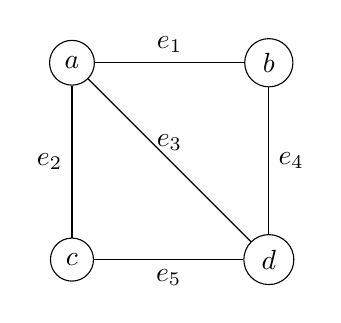
\begin{tikzpicture}[node distance = 2.5cm]
      \node[draw,circle](A) {$a$};
      \node[draw,circle](B) [right of=A] {$b$};
      \node[draw,circle](C) [below of=A] {$c$};
      \node[draw,circle](D) [right of=C] {$d$};
      \draw (A) -- (B) node[midway,above] {$e_1$};
      \draw (A) -- (C) node[midway,left] {$e_2$};
      \draw (A) -- (D) node[midway,above] {$e_3$};
      \draw (B) -- (D) node[midway,right] {$e_4$};
      \draw (C) -- (D) node[midway,below] {$e_5$};
    \end{tikzpicture}
    \end{center}
    \begin{itemize}
    \item[] Example: 
    \item $S = \{a\}, T = \{b,d\}$
    \item $f(S) = |\{e_1, e_2, e_3\}|,~f(T) = |\{e_1, e_3, e_5\}|$
    \item $f(S \cup T) = |\{e_2, e_5\}|,~f(S \cap T) = |\emptyset|$
    \item $\Rightarrow f(S) + f(T) \geq f(S \cup T) + f(S \cap T)$
    \end{itemize}
\end{frame}

  \begin{frame}{Exercise}
    Prove that $f: 2^V \rightarrow \N$ defined by $f(T) = |\delta(T)|$
    for all $T \subseteq V$ is submodular.
  \end{frame}

  %% \begin{itemize}
  %% \item for any $S,T \subseteq V$:
  %% \item let $(T \setminus S : S \setminus
  %%   T)$ be the set of edges with one endnode in $(T \setminus S)$ and
  %%   the other in $(S \setminus T)$
  %% \item $\Rightarrow |\delta(S)| + |\delta(T)| =
  %%   |\delta(S \cap T)| + |\delta(S \cup T)| + 2|(T \setminus S : S
  %%   \setminus T)|$
  %%   \end{itemize}

\begin{frame}{Properties}
  \begin{itemize}
  \item If $a_j \in \R$ for $j \in U$ and $a_0 \in \R$, then $f(T) =
    a_0 + \sum\limits_{j \in T} a_j$ is submodular on $U$
  \item If $f$ is submodular on U and $a \in \R$, then $\bar{f}(T) =
    \min(f(T),a)$ is submodular on $U$
  \item If $f_1$ and $f_2$ are submodular on $U$, then $f(T) = f_1(T)
    + f_2(T)$ is submodular on $U$
  \end{itemize}
\end{frame}

\begin{frame}{Diminishing returns property}
  \begin{definition}
    A set function $f : 2^U \rightarrow \R$ is submodular if \[f(S
    \cup \{i\}) - f(S) \geq f(T \cup \{i\}) - f(T) \] for all $S,T
    \subseteq U$ with $S \subseteq T$ and for all $in \in U \setminus
    T$.
  \end{definition}
\end{frame}

\section{Algorithms to minimize submodular functions}
\begin{frame}{Proposition}
  \begin{prop}\label{prop}
    If $c_J, r_J \geq 0$ for $J \subseteq U$,
    then \begin{equation}f(S) = -\sum\limits_{J \subseteq S} c_J +
      \sum\limits_{J \cap S \neq \emptyset}
      r_J\label{prop}\end{equation} is a submodular function.
  \end{prop}
\end{frame}

\begin{frame}{Proof}
  \begin{proof}
    \begin{align*}
      f(S \cup \{i\}) - f(S) =
%      -\sum\limits_{J \subseteq S \cup \{i\}} c_J + \sum\limits_{J \subseteq S} c_J + &\sum\limits_{J \cap (S \cup \{i\}) \neq \emptyset} r_J - \sum\limits_{J \cap S \neq \emptyset} r_J = \\
      -\sum\limits_{J \subseteq S} c_{J \cup \{i\}} + \sum\limits_{\substack{J: J \cap S = \emptyset,\\i \in J}} r_J.
    \end{align*}
    \begin{itemize}
    \item If $T \supset S$ and $i \not\in T$, then
      \begin{itemize}
      \item $\{J : J \subseteq S\} \subseteq \{J: J \subseteq T\}$ and
      \item $\{J: J \cap T = \emptyset,i\in J\} \subseteq \{J: J \cap S = \emptyset,i \in J\}$.
      \end{itemize}
      \item Hence, $f(S \cup \{i\}) - f(S) \geq f(T \cup \{i\}) -
        f(T)$ for $S \subseteq T$ and $i \in U \setminus T$.
    \end{itemize}
  \end{proof}
\end{frame}

%% \begin{frame}{Exercise}
%%   Write down $f(S \cup \{j\}) - f(S)$ in full detail and comprehend
%%   proof.
%% \end{frame}

\begin{frame}
  \begin{theorem}
    If $f$ is a submodular function of the form
    (\ref{prop}), \[\min\limits_{S \subseteq U} f(S)\] can be solved
    by finding a maximum $s-t$ flow in a digraph $D$ with $n$+2 nodes
    where $n = |\{J \subseteq U: c_J > 0\}| + |\{J \subseteq U: r_J >
    0\}|$.
  \end{theorem}
\end{frame}

%% \begin{frame}{Example}
%%   \begin{itemize}
%%     \item let $G = (V,E)$ be a graph with edge weights $w \in
%%       \R_+^{|E|}$
%%     \item $e \in E$ corresponds to $\{u,v\}$ for $u,v \in V$ with
%%       $u<v$
%%     \item consider $f(S) = |S| - \sum\limits_{e \in E(S)} w_e$ for $S
%%       \subseteq V$
%%     \item define 
%%   \end{itemize}
%%   \begin{minipage}{0.49\textwidth}
%%     \[r_T = \begin{cases} 1 & \text{for}~T \in V\\
%%       0 & \text{otherwise}\end{cases}\]
%%   \end{minipage}
%%   \begin{minipage}{0.49\textwidth}
%%     \[c_T = \begin{cases} w_e & \text{for}~T=e\\
%%       0 & \text{otherwise}\end{cases}\]
%%   \end{minipage}
%%   \begin{itemize}
%%   \item $f(S) = \sum\limits_{T \cap S \neq \emptyset} r_T - \sum\limits_{T \subseteq S} c_T = \sum\limits_{j \in S} 1 - \sum\limits_{e \in E(S)} w_e$
%%   \end{itemize}
%% \end{frame}

\begin{frame}{Proposition for the non-empty case}
  Consider \begin{equation}\min\limits_{\emptyset \neq S \subseteq U}
    f(S)\label{non-empty}\end{equation} where $f$ is submodular.
  \begin{prop}
    Problem (\ref{non-empty}) can be solved by solving $\min\limits_{S
      \subseteq U} f(S)$ no more than $|U|$ times.
  \end{prop}
  \begin{proof}
    Since $S \neq \emptyset$, it follows that $j \in S$ for some $j
    \in U$. Define $U_j = U \setminus \{j\}$ and $f_j(T) = f(T \cup
    \{j\})$ for $j \in U$. Note that $f_j$ is submodular. Then it
    suffices to solve \[\min\limits_{T \subseteq U_j}
    f_j(T)~~\text{for}~j \in U.\]
  \end{proof}
\end{frame}

\begin{frame}{Back to Steiner tree polytope}
  \begin{itemize}
  \item let $N = V \setminus T$ be the set of non-terminals
  \item $x_e \in \{0,1\}$ for $e \in E$ with $x_e = 1$ iff  $e$ is used in Steiner tree
  \item $y_i \in \{0,1\}$ for $i \in N$ iff vertex $i$ is spanned by the Steiner tree
  \item[]
  \item $\sum\limits_{e \in E(S)} x_e \leq \sum\limits_{i \in N \cap S} y_i + |T \cap S| -1~~\forall S \subseteq V,~S \cap T \neq \emptyset$
  \item[]
  \item $f(S) =  \sum\limits_{i \in N \cap S} y_i + \sum\limits_{i \in T \cap S} 1 - 1 - \sum\limits_{e \in E(S)} x_e$
  \item[]
    \item we want to solve $\min\limits_{\substack{S \subseteq V\\S \cap T \neq \emptyset}} f(S)$
  \end{itemize}
%  \begin{align*}f(S)
%    = &\sum\limits_{i \in N \cap S} y_i + |T \cap S| - \sum\limits_{e \in E(S)} x_e
%    =  &\sum\limits_{i \in N \cap S} y_i + \sum\limits_{i \in T \cap S} 1 - \sum\limits_{e \in E(S)} x_e\end{align*}
\end{frame}



\begin{frame}{$S \subseteq V, S \cap T \neq \emptyset$}
  \begin{itemize}
  \item let $i \in T$ and $S \subseteq V \setminus \{i\}$
  \end{itemize}
  \begin{align*}f(S \cup \{i\}) &= \sum\limits_{j \in N \cap (S \cup \{i\})} y_j + \sum\limits_{j \in T \cap (S \cup \{i\})} 1 - 1 - \sum\limits_{e \in E(S \cup \{i\})} x_e \\
    &= \sum\limits_{j \in N \cap S} y_j + \sum\limits_{j \in T \cap S} 1 - \sum\limits_{e \in E(S \cup \{i\})} x_e \\
    &= g_i(S)
  \end{align*}
\end{frame}

\begin{frame}{Show $g_i$ is submodular}
  \begin{minipage}{0.49\textwidth}
    \[r_J = \begin{cases} y_J & \text{for}~J \in N\\
      1 & \text{for}~J \in T\\ 0 & \text{otherwise}\end{cases}\]
  \end{minipage}
  \begin{minipage}{0.49\textwidth}
    \[c_J = \begin{cases} x_{e} & \text{for}~J=e \\
      x_{\{i,J\}} & \text{for}~J \in V \\
      0 & \text{otherwise}\end{cases}\]
  \end{minipage}
  \begin{align*}
    g_i(S) &= \sum\limits_{J \cap S \neq \emptyset} r_J - \sum\limits_{J \subseteq S} c_J \\
    &= \sum\limits_{j \in N \cap S} y_j + \sum\limits_{j \in T \cap S} 1 - \sum\limits_{e \in E(S)} x_e - \sum\limits_{j \in S} x_{\{i,j\}} \\
    &= \sum\limits_{j \in N \cap S} y_j + \sum\limits_{j \in T \cap S} 1 - \sum\limits_{e \in E(S \cup \{j\})} x_e
  \end{align*}
\end{frame}

%% \begin{frame}{Show $f(S)$ is of the form (\ref{prop})}
%%   \begin{minipage}{0.49\textwidth}
%%     \[r_J = \begin{cases} y_J^* & \text{for}~J \in N\\
%%       1 & \text{for}~J \in T\\ 0 & \text{otherwise}\end{cases}\]
%%   \end{minipage}
%%   \begin{minipage}{0.49\textwidth}
%%     \[c_J = \begin{cases} x^*_e & \text{for}~J=e\\
%%       0 & \text{otherwise}\end{cases}\]
%%   \end{minipage}
%%   \[f(S)
%%   = \sum\limits_{J \cap S \neq \emptyset} r_J - \sum\limits_{J \subseteq S} c_J
%%   = \sum\limits_{i \in N \cap S} y^*_i + \sum\limits_{i \in T \cap S} 1 - \sum\limits_{e \in E(S)} x^*_e\]
%%   \begin{itemize}
%%     \item $\Rightarrow~f(S)$ is submodular
%%     \item we want to solve $\min\limits_{\substack{S \subseteq V,\\S
%%         \cap T \neq \emptyset}} f(S)$
%%   \end{itemize}
%% \end{frame}

\begin{frame}{Solve via maximum flow in directed graph}
  \begin{itemize}
  \item consider digraph $D = (V_1 \cup V_2 \cup \{s,t\}, A)$ where
    \item $V_1 = \{J \subseteq U: c_J > 0\}$
    \item $V_2 = \{J \subseteq U: r_J > 0\}$
    \item $A = \{(I,J) : I \in V_1,~J \in V_2, I \cap J \neq
      \emptyset\} \cup \{(s, J) : J \in V_1\} \cup \{(J, t): J \in
      V_2\}$
    \item with capacities $d_a$ for $a \in A$ where
      \begin{itemize}
      \item $d_a = \infty$ for $a = (I,J)$
      \item $d_a = c_J$ for $a = (s,J)$
      \item $d_a = r_J$ for $a = (J,t)$
      \end{itemize}
  \end{itemize}
\end{frame}

\begin{frame}{Min s-t cuts}
  \begin{prop}
    Every minimal s-t cut $(W_1, W_2)$ in $D$ can be characterised by
    a set $R \subseteq U$ where $W_1 = \{J \in V_1: J \subseteq R\}$
    and $W_2 = \{J \in V_2: J \cap R \neq \emptyset\}$. The cut has
    capacity \[d(W_1, W_2) = d(R) = \sum\limits_{J \cap (U \setminus
      R) \neq \emptyset} c_J + \sum\limits_{J \cap R \neq \emptyset}
    r_J.\]
  \end{prop}
It holds that  \[d(R) = \sum\limits_{J \subseteq U} c_J - \sum\limits_{J \subseteq R} c_J + \sum\limits_{J \cap R \neq \emptyset} r_J = f(R) + \sum\limits_{J \subseteq U} c_J.\]
\end{frame}

\section{Example}
\begin{frame}[fragile]{Example instance - Optimal solution}
  \begin{minipage}{0.49\textwidth}
  \verbatiminput{example_graph.txt}
  \end{minipage}
  \begin{minipage}{0.49\textwidth}
    \begin{center}
    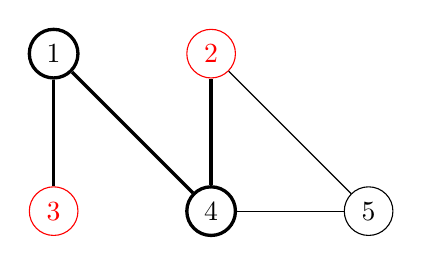
\begin{tikzpicture}[node distance = 2cm]
    \node[draw,circle, very thick](1) {$1$};
    \node[draw,circle, red](2) [right of=1] {$2$};
    \node[draw,circle, red](3) [below of=1] {$3$};
    \node[draw,circle, very thick](4) [right of=3] {$4$};
    \node[draw,circle](5) [right of=4] {$5$};
    \draw[very thick] (1) -- (3);
    \draw[very thick] (1) -- (4);
    \draw[very thick] (2) -- (4);
    \draw[] (2) -- (5);
    \draw[] (4) -- (5);
    \end{tikzpicture}
    \end{center}
  \end{minipage}
\end{frame}

\begin{frame}{LP relaxation}
  \begin{minipage}{0.49\textwidth}
    \begin{align*}
      \max &\sum_{i \in N} p_i y_i~~\textbf{s.t.}\\
      &\sum\limits_{i \in N} w_i y_i + |T| \leq b\\
      &\sum\limits_{e \in E} x_e = \sum\limits_{i \in N} y_i + |T| - 1\\
      &x_e \geq 0~~\forall e \in E\\
      &y_i \leq 1~~\forall i \in N
    \end{align*}
  \end{minipage}
  \begin{minipage}{0.49\textwidth}
    \begin{center}
    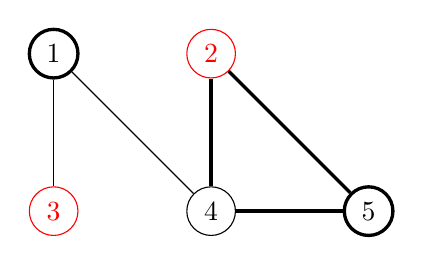
\begin{tikzpicture}[node distance = 2cm]
      \node[draw,circle, very thick](1) {$1$};
      \node[draw,circle, red](2) [right of=1] {$2$};
      \node[draw,circle, red](3) [below of=1] {$3$};
      \node[draw,circle](4) [right of=3] {$4$};
      \node[draw,circle, very thick](5) [right of=4] {$5$};
      \draw (1) -- (3);
      \draw (1) -- (4);
      \draw[very thick] (2) -- (4);
      \draw[very thick] (2) -- (5);
      \draw[very thick] (4) -- (5);
    \end{tikzpicture}
  \end{center}
  \begin{itemize}
  \item $x_{24}, x_{25}, x_{45} = 1$
  \item $y_1, y_5 = 1$
  \end{itemize}
  \end{minipage}
\end{frame}

\begin{frame}{Violated inequality}
  \begin{itemize}
  \item $\sum\limits_{e \in E(S)} x_e \leq \sum\limits_{i \in N \cap S} y_i + |T \cap S| - 1~~\forall S \subseteq V,~S \cap T \neq \emptyset$
  \end{itemize}
  \vspace{1cm}
  \begin{minipage}{0.49\textwidth}
    \begin{center}
    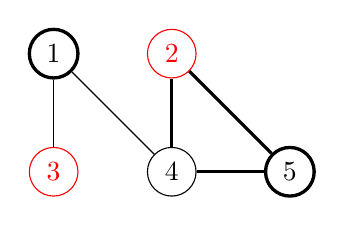
\begin{tikzpicture}[node distance = 1.5cm]
    \node[draw,circle, very thick](1) {$1$};
    \node[draw,circle, red](2) [right of=1] {$2$};
    \node[draw,circle, red](3) [below of=1] {$3$};
    \node[draw,circle](4) [right of=3] {$4$};
    \node[draw,circle, very thick](5) [right of=4] {$5$};
    \draw (1) -- (3);% node[midway,left] %{$e_{13}$};
    \draw (1) -- (4);% node[midway,above] {$e_{14}$};
    \draw[very thick] (2) -- (4);% node[midway,right] {$e_{24}$};
    \draw[very thick] (2) -- (5);% node[midway,below] {$e_{25}$};
    \draw[very thick] (4) -- (5);% node[midway,below] {$e_{45}$};
    \end{tikzpicture}
  \end{center}
  \end{minipage}
  \begin{minipage}{0.49\textwidth}
    \begin{itemize}
    \item for $S = \{2,4,5\}$
      \begin{itemize}
      \item $\sum\limits_{e \in E(S)} x_e = 3$
      \item $\sum\limits_{i\in N \cap S} y_i + |T \cap S| - 1 = 1$
      \end{itemize}
        \item $\Rightarrow x_{24} + x_{25} + x_{45} \leq y_4 + y_5$
    \end{itemize}
  \end{minipage}
\end{frame}

\begin{frame}{Solve $\min_{S \subseteq V \setminus \{2\}} g_2(S)$}
  \begin{itemize}
  \item considered solution: $x_{24}, x_{25}, x_{45}, y_1, y_5 = 1$
  \end{itemize}
  \begin{center}
    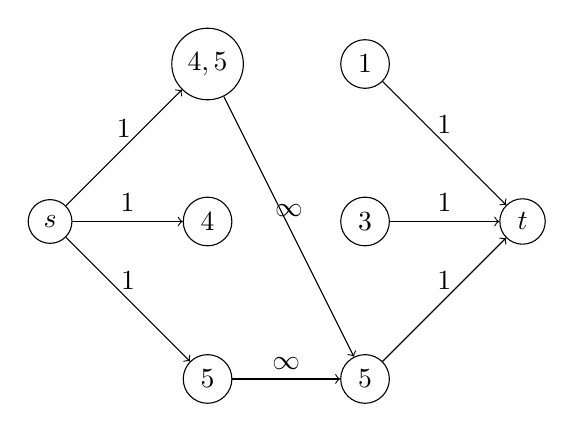
\begin{tikzpicture}[node distance = 2cm]
      \node[draw,circle](s) {$s$};
      \node[draw,circle](B) [right of=s] {$4$};
      \node[draw,circle](A) [above of=B] {$4,5$};
      \node[draw,circle](C) [below of=B] {$5$};
      \node[draw,circle](E) [right of=B] {$3$};
      \node[draw,circle](D) [above of=E] {$1$};
      \node[draw,circle](F) [below of=E] {$5$};
      \node[draw,circle](t) [right of=E] {$t$};
      \draw[->] (s) -- (A) node[midway,above] {$1$};
      \draw[->] (s) -- (B) node[midway,above] {$1$};
      \draw[->] (s) -- (C) node[midway,above] {$1$};
      \draw[->] (A) -- (F) node[midway,above] {$\infty$};
      \draw[->] (C) -- (F) node[midway,above] {$\infty$};
      \draw[->] (D) -- (t) node[midway,above] {$1$};
      \draw[->] (E) -- (t) node[midway,above] {$1$};
      \draw[->] (F) -- (t) node[midway,above] {$1$};
    \end{tikzpicture}
  \end{center}
  \begin{itemize}
  \item $R = \{4,5\}$
  \item $g_2(R) = d(R) - \sum\limits_{J \subseteq U \setminus \{2\}}
    c_J = -2$
  \end{itemize}
\end{frame}

\begin{frame}{References}
  \begin{itemize}
  \item Goemans, Myung: "A catalog of Steiner tree formulations"
  \item Nemhauser, Wolsey: "Integer and combinatorial optimization"
  \end{itemize}
\end{frame}

\end{document}
 
